\documentclass[tikz,border=1cm]{standalone}
\usepackage{amsmath}
\usepackage{amssymb}
\usetikzlibrary{arrows.meta}
\usetikzlibrary{positioning}
\begin{document}
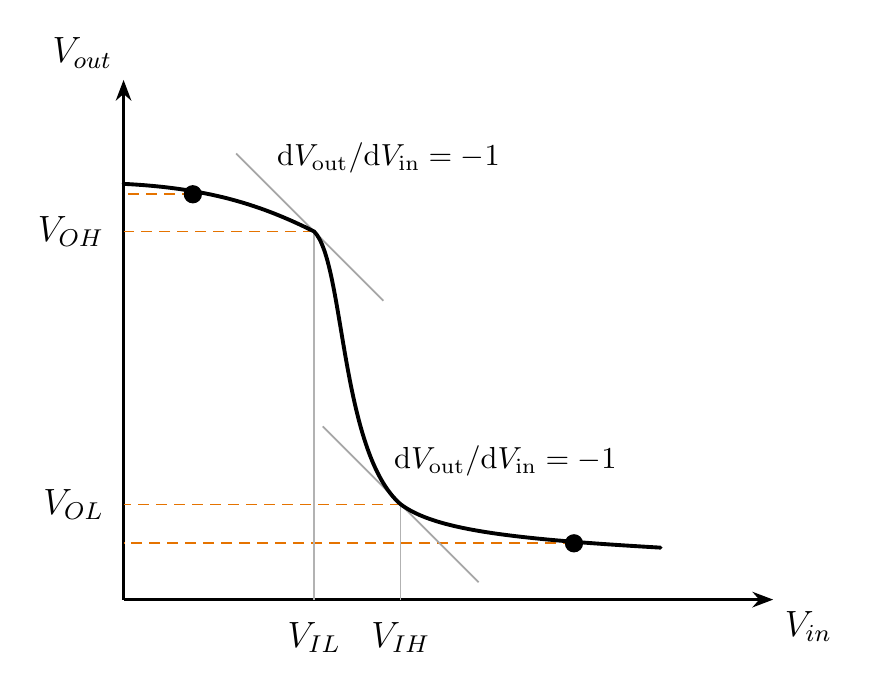
\begin{tikzpicture}[>=Stealth, scale=1.1, every node/.style={transform shape}]
  % 坐标轴
  \draw[->, line width=1.0pt] (0, 0) -- (7.5, 0) node[below right, font=\large] {$V_{in}$};
  \draw[->, line width=1.0pt] (0, 0) -- (0, 6.0) node[above left, font=\large] {$V_{out}$};

  % 辅助黄色/橙色虚线
  \draw[dashed, orange!90!black, line width=0.6pt, dash pattern=on 4pt off 2.5pt] (0.8, 4.68) -- (0, 4.68);
  \draw[dashed, orange!90!black, line width=0.6pt, dash pattern=on 4pt off 2.5pt] (2.2, 4.25) -- (0, 4.25);
  \draw[dashed, orange!90!black, line width=0.6pt, dash pattern=on 4pt off 2.5pt] (3.2, 1.1) -- (0, 1.1);
  \draw[dashed, orange!90!black, line width=0.6pt, dash pattern=on 4pt off 2.5pt] (5.2, 0.65) -- (0, 0.65);

  % 辅助灰色垂直投影实线
  \draw[gray!60, line width=0.5pt] (2.2, 4.25) -- (2.2, 0);
  \draw[gray!60, line width=0.5pt] (3.2, 1.1) -- (3.2, 0);

  % 坐标轴刻度标签
  \node[left=3pt, font=\large\bfseries] at (0, 4.25) {$V_{OH}$};
  \node[left=3pt, font=\large\bfseries] at (0, 1.1) {$V_{OL}$};
  \node[below=4pt, font=\large\bfseries] at (2.2, 0) {$V_{IL}$};
  \node[below=4pt, font=\large\bfseries] at (3.2, 0) {$V_{IH}$};

  % 切线 (斜率 = -1)
  \draw[gray!70, line width=0.6pt] (1.3, 5.15) -- (3.0, 3.45);
  \node[above right, font=\normalsize] at (1.65, 4.8) {$\mathrm{d}V_{\mathrm{out}}/\mathrm{d}V_{\mathrm{in}} = -1$};

  \draw[gray!70, line width=0.6pt] (2.3, 2.0) -- (4.1, 0.2);
  \node[above right, font=\normalsize] at (3.0, 1.3) {$\mathrm{d}V_{\mathrm{out}}/\mathrm{d}V_{\mathrm{in}} = -1$};

  % VTC 特性曲线 (平滑贝塞尔曲线，过渡区陡峭)
  \draw[line width=1.4pt, line cap=round] 
    (0, 4.8) 
    .. controls (1.0, 4.75) and (1.6, 4.55) .. (2.2, 4.25)
    .. controls (2.55, 3.9) and (2.5, 1.7) .. (3.2, 1.1)
    .. controls (3.6, 0.8) and (4.5, 0.7) .. (6.2, 0.6);

  % 状态点 (实心黑色圆点)
  \fill (0.8, 4.68) circle (3pt);
  \fill (5.2, 0.65) circle (3pt);
\end{tikzpicture}

\end{document}
